\section{method}


\hfill \break
\hfill \break
\subsection*{latest writing}
\hfill \break
\hfill \break

Three parts:
A. Extracting semantics using tags from individual images, which is what we did in WWW paper. Discuss simple keyword search on e.g. a few snow words, or machine learning to find keyword combinations. 

B. Extracting semantics using images from individual images. Here we talk about the traditional features that are covered in ICCV paper, and then the deep learning techniques.

C. Combining evidence together across users. Here we have the simple voting method and the probabilistic confidence score. We can augment with the additional factors that Stefan suggested, including priors based on time of year or geographic location, or other evidence like historical accuracy of specific users.] Also including temporal and spatial smoothing by simply adding to the confidence score priors.

[Note what I am omitting here. My preference would be to ignore any techniques that try to classify bins jointly by aggregating all the tags or visual features of photos together in a bin and then using those features. I would also really like if the final classification is based just on thresholding a confidence score, even if the results are slightly worse than the best we can do. I just think it makes the story more complicated to do otherwise and harder to justify.] 

\hfill \break
\hfill \break
===================================
\hfill \break
\hfill \break

\subsubsection*{Vision model}
For each ecology phenomenon, the most descriptive visual features are extracted from images in training set. We test models built from each feature on testing set. Then these features are normalized and concatenated to build a descriptor of each image. With this combined feature, we learn a vision model on training images. This is the model we use to classify an image as having the phenomenon on it or not.

\subsubsection*{Deep learning}


In this convolutional neural network, we use ImageNet pre-trained model, and further tune it with our hand-labeled snow/vege dataset.

\hfill \break
\hfill \break
===================================
\hfill \break
\hfill \break
\subsection*{workshop}


\hfill \break
\hfill \break
===================================
\hfill \break
\hfill \break
\subsection*{www}


%\subsection{Datasets}

We use a sample of nearly 150 million geo-tagged, timestamped Flickr
photos as our source of user-contributed observational data about the
world. We collected this data using the public Flickr API, by
repeatedly searching for photos within random time periods and
geo-spatial regions, until the entire globe and all days between January 1, 2007 and December 31, 2010 had been covered.
We applied filters to remove blatantly inaccurate
metadata, in particular removing photos with geotag precision less
than about city-scale (as reported by Flickr), and photos whose upload
timestamp is the same as the EXIF camera timestamp (which usually
means that the camera timestamp was missing).  

For ground truth we use large-scale data originating from two
independent sources: ground-based weather stations, and aerial
observations from satellites.  For the ground-based observations, we
use publicly-available daily snowfall and snow depth observations from
the U.S. National Oceanic and Atmospheric Administration (NOAA) Global
Climate Observing System Surface Network (GSN)~\cite{ghcn}.  This data
provides highly accurate daily data, but only at sites that have
surface observing stations. 
%
For denser, more global coverage, we also use
data from the Moderate Resolution Imaging Spectroradiometer (MODIS)
instrument aboard NASA's Terra satellite. The satellite is in a polar
orbit so that it scans the entire surface of the earth every day. The
MODIS instrument measures spectral emissions at various wavelengths,
and then post-processing uses these measurements to estimate ground cover.
In this paper we use two datasets: the daily snow cover
maps~\cite{modissnow} and the two-week vegetation
averages~\cite{modisveg}. Both of these sets of data including an
estimate of the percentage of snow or vegetation ground cover at each
point on earth, along with a quality score indicating the confidence
in the estimate. Low confidence is caused primarily by cloud cover
(which changes the spectral emissions and prevents accurate ground
cover from being estimated), but also by technical problems with the
satellite. 
As an example, Figure~\ref{fig:samplemap} shows raw satellite snow data from one particular day.




%% \begin{figure}
%% \begin{center}
%% \begin{tabular}{cc}
%% 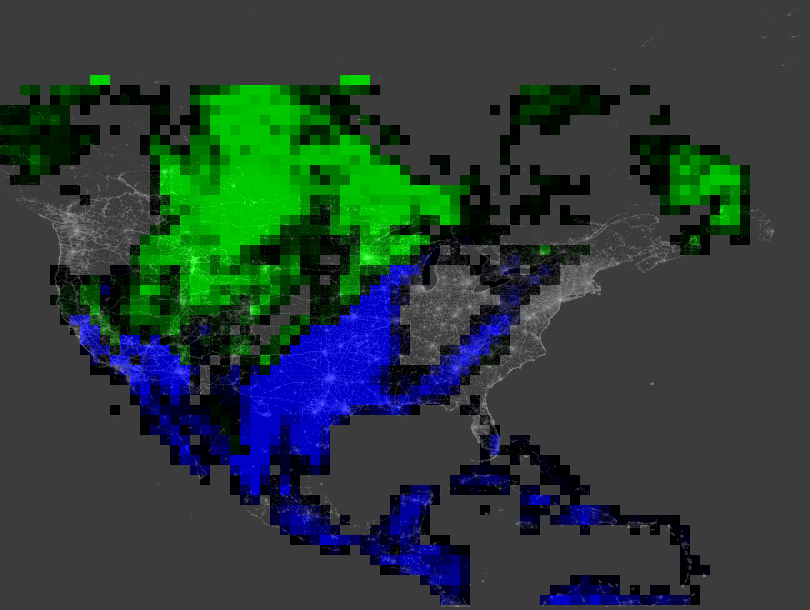
\includegraphics[width=0.5\textwidth]{plots/nasadownsample20070101.png}
%% \end{tabular}
%% \end{center}
%% \caption{Down-sampled NASA MODIS snow coverage data for North America
%%   on 2007.01.01. Grey: water-covered, or no data, or the confidence
%%   index value is 0; blue: no snow and has non-zero confidence index
%%   value; green: has snow and non-zero confidence index value. (Please
%%   view in color.)}
%% \label{fig:nasadownsample20070101}
%% \end{figure}


\subsection{Estimation techniques}
\label{sec:methods}

Our goal is to estimate the presence or absence of a given ecological
phenomenon (like a species of plant or flower, or a meteorological
feature like snow) on a given day and at a given place,
using only the geo-tagged, time-stamped photos from Flickr. One way of viewing
this problem is that every time a user takes a photo of a phenomenon
of interest, they are casting a ``vote''  that the
phenomenon actually occurred in a given geospatial region. 
 We could
simply look for tags indicating the presence of a feature --
i.e. count the number of photos with the tag ``snow'' --  
but sources of noise and bias make this task 
challenging, including:
\begin{packed_itemize}
\item[---] \textit{Sparse sampling:} The geospatial distribution of photos
  is highly non-uniform. A lack of photos
  of a phenomenon in a region does not
  necessarily mean that it was not there. 
\item[---] \textit{Observer bias:} Social media users are younger and
  wealthier than average, and most live in North
  America and Europe.
\item[---] \textit{Incorrect, incomplete and misleading tags:}
  Photographers may use incorrect or ambiguous tags  ---
  e.g. the tag ``snow'' may refer to a snowy owl or interference on a
  TV screen.
\item[---] \textit{Measurement errors:} Geo-tags and timestamps are
  often incorrect (e.g. because people   forget to set their camera clocks).
\end{packed_itemize}

\xhdr{A statistical test.}  We introduce a simple probabilistic model
and use it to derive a statistical test that can deal with some such
sources of noise and bias. The test could be used for estimating the
presence of any phenomenon of interest; without loss of generality we
use the particular case of snow here, for ease of explanation.  Any
given photo either contains evidence of snow (event $s$) or does not
contain evidence of snow (event $\bar{s}$).  We assume that a given
photo taken at a time and place with snow has a fixed probability $P(s
| snow)$ of containing evidence of snow; this probability is less than
1.0 because many photos are taken indoors, and outdoor photos might be
composed in such a way that no snow is visible. We also assume that
photos taken at a time and place without snow have some non-zero
probability $P(s | \overline{snow})$ of containing evidence of snow;
this incorporates various scenarios including incorrect timestamps or
geo-tags and misleading visual evidence (e.g.  man-made
snow).

Let $m$ be the number of snow
photos (event $s$), and $n$ be the number of non-snow photos (event
$\bar{s}$) taken at a place and time of interest. Assuming that each photo is captured
independently, we can use Bayes' Law to
derive the probability that a given place has snow
given its number of snow and non-snow photos,
%
%\newcommand{\smsn}{\overbrace{s\cdots s}^{m},\overbrace{\overline{s}\cdots \overline{s}}^{n}}
%%hp cr: \bar{s}^n
\newcommand{\smsn}{s^m, \bar{s}^n}
\newcommand{\smsntwo}{s^m, \bar{s}^n}
%%\newcommand{\smsn}{s^m, s^n}
%%\newcommand{\smsntwo}{s^m, s^n}
%\newcommand{\smsntwo}{\underbrace{s\cdots s}_{m},\underbrace{\overline{s}\cdots \overline{s}}_{n}}
\begin{eqnarray*}
P(snow|\smsn)  &=&\frac{ P(\smsn|snow)P(snow)}{P(\smsntwo)}  \\
&=&\frac{{m+n\choose m}p^{m}(1-p)^{n}P(snow)}{P(\smsntwo)},  
\end{eqnarray*}
%
where we write $s^m, \bar{s}^n$ to denote $m$ occurrences of event $s$ and $n$ occurrences of event $\bar{s}$, and where $p=P(s|snow)$ and $P(snow)$ is the prior probability of snow. A similar derivation gives the posterior probability that the bin does not contain snow,
%
\begin{eqnarray*}
P(\overline{snow}|\smsn)  &=&\frac{{m+n\choose m}q^{m}(1-q)^{n}P(\overline{snow})}{P(\smsntwo)},  
\end{eqnarray*}
%
where $q=P(s|\overline{snow})$. 
%
Taking the ratio between these two posterior probabilities yields a likelihood ratio,
%
\begin{eqnarray}
\frac{P(snow|\smsn)}{P(\overline{snow}|\smsntwo)}
%\\=\frac{\frac{{m+n\choose m}p^{m}(1-p)^{n}P(snow)}{P(\overbrace{s\cdots s}^{m},\overbrace{\overline{s}\cdots \overline{s}}^{n})}}{\frac{{m+n\choose m}q^{m}(1-q)^{n}P(\overline{snow})}{P(\overbrace{s\cdots s}^{m},\overbrace{\overline{s}\cdots \overline{s}}^{n})}}
&=&\frac{P(snow)}{P(\overline{snow})}\left(\frac{p}{q}\right)^{m}\left(\frac{1-p}{1-q}\right)^n.
\label{eq:conf}
\end{eqnarray}
%
This ratio can be thought of as a measure of the confidence that a
given time and place actually had snow, given photos from Flickr.

A simple way of classifying a photo into a positive event $s$ or a
negative event $\bar{s}$ is to use text tags. We identify a
set ${\cal S}$ of tags related to a phenomenon of
interest. Any photo tagged with at least one tag in ${\cal S}$ is
declared to be a positive event $s$, and otherwise it is considered a
negative event $\bar{s}$. For the snow detection task, we use the set
${\cal S}$=\{snow, snowy, snowing, snowstorm\}, which we selected
by hand.

%%, which we chose by
%%looking at the 200 most frequent Flickr tags and hand selecting those
%%directly relevant to snowfall.

The above derivation assumes that photos are taken independently of
one another, which is generally not true in reality. One particular
source of dependency is that photos from the same user are highly
correlated with one another.  To mitigate this problem, instead of
counting $m$ and $n$ as numbers of \textit{photos}, we instead let $m$ be 
the number of \textit{photographers} having at least one photo with evidence of snow,
while $n$ is the numbers of photographers who did not upload any
photos with evidence of snow.

The probability parameters in the likelihood ratio of
equation~(\ref{eq:conf}) can be directly estimated from training data
and ground truth. For example, for the snow cover results
presented in Section~\ref{sec:results}, the learned parameters are: $p
= p(s|snow) = 17.12\%$, $q = p(s|\overline{snow}) = 0.14\%$.  In other
words, almost 1 of 5 people at a snowy place take a photo containing
snow, whereas about 1 in 700 people take a photo containing evidence
of snow at a non-snowy place.

Figure~\ref{fig:samplemap} shows a visualization of the likelihood
ratio values for the U.S. on one particular day using this simple
technique with ${\cal S}$=\{snow, snowy, snowing, snowstorm\}.  High
likelihood ratio values are plotted
in green, indicating a high confidence of snow in a geospatial bin,
while low values are shown in blue and indicate high confidence of 
no snow.  Black areas indicate a likelihood ratio 
near 1, showing little conference either way, and grey areas lack
data entirely (having no Flickr photos in that bin on that day).

\subsection{Learning features automatically}

The confidence score in the last section has a number of limitations,
including requiring that a set of tags related to the phenomenon of
interest be selected by hand. Moreover, it makes no attempt to
incorporate visual evidence or negative textual evidence --- e.g.,
that a photo tagged ``snowy owl'' probably contains a bird and no
actual snow.  We use machine learning techniques to address these
weaknesses, both to automatically identify specific tags and tag
combinations that are correlated with the presence of a phenomenon of
interest, and to incorporate visual evidence into the prediction techniques.

\xhdr{Learning tags.}  We consider two learning paradigms. The first
is to produce a single exemplar for each bin in time and space
consisting of the set of all tags used by all users. For each of these
exemplars, the NASA and/or NOAA ground truth data gives a label (snow
or non-snow). We then use standard machine learning algorithms like
Support Vector Machines and decision trees to identify the most
discriminative tags and tag combinations. In the second paradigm, our
goal instead is to classify individual \textit{photos} as containing
snow or not, and then use these classifier outputs to compute the
number of positive and non-positive photos in each bin (i.e., to
compute $m$ and $n$ in the likelihood ratio described in the last
section).

\xhdr{Learning visual features.}  We also wish to incorporate visual
evidence from the photos themselves. There is decades of
work in the computer vision community on object and scene
classification (see~\cite{szeliski} for a recent survey), although
most of that work has not considered the large, noisy photo collections we work with here. We tried a number of
approaches, and found that a classifier using a simplified version of
GIST  augmented with color features~\cite{gist, hays}
gave a good trade-off between accuracy and 
tractability.

\newcommand{\lab}{CIELAB }
Given an image $I$, we partition the image into a $4 \times 4$ grid of
16 equally-sized rectangular regions. In each region we compute the
average pixel values in each of the red, green, and blue color planes,
and then convert this color triple from sRGB space to the \lab color
space~\cite{lab}. \lab  has a number of advantages, including
separating greyscale intensity from the color channels and having greater
perceptual uniformity (so that Euclidean distances between two \lab
color triples are approximately proportional to the human perception
of difference between the colors). For each region $R$ we also compute the
total gradient energy $E(R)$ within the grayscale plane $I_g$ of the image,
%
\begin{eqnarray*}
E(R) & = & \sum_{(x,y) \in R}   || \nabla I_g(x,y) || \\
& = & \sum_{(x,y) \in R} \sqrt{I_x(x,y)^2 + I_y(x,y)^2}, 
\end{eqnarray*}
%
where $I_x(x,y)$ and $I_y(x,y)$ are the partial derivatives in the $x$
and $y$ directions evaluated at point $(x,y)$, approximated as,
%
\begin{eqnarray*}
I_x(x,y) = I_g(x+1, y) - I_g(x-1, y), \\
 I_y(x,y) = I_g(x, y+1) - I_g(x, y-1).
\end{eqnarray*}
%
  For each image we
concatenate the gradient energy in each of the 16 bins, followed by
the 48 color features (average L, a, and b values for each of the 16
bins), to produce a 64-dimensional feature vector.  We then learn a
Support Vector Machine (SVM) classifier from a labeled training image
set.
